\chapter{La Gestion des Stocks}\label{chap:gestion-stocks}
\index{la gestion des stocks}

\utilisateurs: \liencaissier, \liengestionnairedesstocks,
			   \lienmagasinier, \lienmanager, \lienvendeur.\\

\chapintro{Ce chapitre d\'ecrit comment avoir acc\`es aux
fonctionalit\'es de gestion des stocks et comment les utiliser.}

\nxsection{Introduction}

Les t\^aches de gestion des stocks sont illustr\'ees
dans le Tableau~\ref{tab:taches-fonctions}, en fonction
du r\^ole de l'utilisateur.\\

\begin{table}[!htbp]
\centering
\begin{tabular}{lccccc}
\textbf{T\^aches} 							& \managerb		 & \vendeurb	 		&	\gestionairedestocksb	& \magasinierb		& \caissierb 		\\ \hline
acc\'eder aux  	& 				 &				 		&				 			& 					&  				 	\\ 
mouvements des stocks 	   		 			& \mytimes{blue} & 				 		&\mytimes{blue}				& \mytimes{blue}  	& \\ \hline
afficher les d\'etails d'un stock 			& \mytimes{blue} & 	\mytimes{blue} 		& \mytimes{blue}			& \mytimes{blue}	&  				 	\\ \hline
afficher l'historique d'un stock 			& \mytimes{blue} & 	\mytimes{blue} 		& \mytimes{blue}			& 					&		\\ \hline
entrer un stock 							& \mytimes{blue} & 				 		& \mytimes{blue}			& 					&  				 	\\ \hline
lister les stocks 							& \mytimes{blue} &\mytimes{blue} 		& \mytimes{blue}			& \mytimes{blue}	& \mytimes{blue} 	\\ \hline
modifier la strat\'egie 					&  				 & 				 		& 							& 					&	 				\\ 
de gestion des stocks  						& \mytimes{blue} & \mytimespartial{blue}& \mytimespartial{blue}		& 					&  				 	\\ 
(ex.: \fifo, etc.)							&				 &				 		&							&					&					\\ \hline
modifier un stock 							& \mytimes{blue} & 				 		& \mytimes{blue}			& 					&  				 	\\ \hline

supprimer un stock 							& \mytimes{blue} & 				 		& 							&					&  					\\ \hline

transf\'erer des stocks 					& \mytimes{blue} & 				 		& \mytimes{blue}			& \mytimes{blue}	&  				 	\\ \hline
sortir des stocks							& \mytimes{blue} & 				 		& \mytimes{blue}			& \mytimes{blue}	&  				 	\\
\end{tabular}
\caption{Tableau des t\^aches et des r\^oles associ\'es
\`a la gestion des stocks}
\label{tab:taches-fonctions}
\index{t\^aches de gestion des stocks}
\end{table}

\nxsection{Les strat\'egies de gestion des stocks}\label{sec:strategies-gestion-stocks}
\index{strat\'egies de gestion des stocks}
\index{strat\'egie de sortie des articles}
\index{strat\'egie de vente des articles}
\index{strat\'egie de gestion des stocks ! \cmup}
\index{strat\'egie de gestion des stocks ! \dpfdpo}
\index{strat\'egie de gestion des stocks ! \fifo}
\index{strat\'egie de gestion des stocks ! \lifo}

\yeren impl\'emente $4$ strat\'egies pour g\'erer les stocks \`a
vendre ou \`a sortir:
\begin{enumerate}[1)]
	\item \cmup: Cours Moyen, Unit\'e Pond\'er\'ee.
	
		La strat\'egie \cmup affiche tous les 
		stocks de \facon (Cours
		Moyen, Unit\'e Pond\'er\'ee).\\
		
	\item \dpfdpo: Date of Expiration First, Date of Expiration Out.
	
		La strat\'egie \dpfdpo affiche les
		stocks \`a vendre ou \`a sortir selon
		le principe: les stocks avec des dates
		de p\'eremption les plus proches sont 
		les premiers \`a sortir.\\
		
	\item \fifo: First In, First Out. 
	
		La strat\'egie \fifo affiche les stocks
		\`a vendre ou \`a sortir selon le principe
		''\textbf{First In, First Out}'':
		Les stocks avec des dates d'entr\'ee en stock
		plus anciennes sont les premiers \`a sortir.\\
		
	\item \lifo: Last In, First Out.
	
		La strat\'egie \lifo affiche les stocks
		\`a vendre ou \`a sortir selon le principe
		''\textbf{Last In, First Out}'': 
		Les stocks avec des dates d'entr\'ee en stock
		plus r\'ecentes sont les premiers \`a sortir.\\
\end{enumerate}
\index{\cmup}
\index{\dpfdpo}
\index{\fifo}
\index{\lifo}

La strat\'egie de gestion des stocks se modifie
comme suit:

\begin{itemize}[\mycheckmark{purplish}]
	\item de \facon permanente dans
		la section 'administration' de \yerenpos.

	\item de \facon temporaire (\`a des fins de
		visualitation de l'ordre des sorties de
		stocks) dans la \fenetre 
		\textbf{'fiche des stocks'} de \yerenpos.
\end{itemize}

%\newpage

%-----------------------------------------------------------

\nxsection{Entrer un stock}
\index{entrer un stock}
\index{stock minimum}

\yeren entretient les donn\'ees suivantes pour chaque stock:
\begin{enumerate}[1)]
	\item la cat\'egorie \obligatoire
	\item la d\'esignation \obligatoire
	\item la date de p\'eremption du stock 
	\item le fournisseur 
	\item la localisation du stock
	\item le montant de la TVA d'un article 
	\item le prix de vente d'un article \obligatoire
	\item la quantit\'e intiale (nombre de lots, et quantit\'e par lot) \obligatoire
	\item la \reference
	\item la \reference du re\c{c}u d'achat
	\item le stock minimum: si cette quantit\'e
		est atteinte, alors le nombre de la colone 'Qt\'e totale'
		du stock est affich\'e en rouge.\\
\end{enumerate}

Il existe deux m\'ethodes pour entrer un stock dans \yeren:
\begin{enumerate}[1)]
	\item la $\mathbf{1^{\textbf{\`ere}}}$ \textbf{m\'ethode}
	est utilis\'ee pour entrer un stock d'articles \`a partir
	d'un formulaire vide
	
	\item la $\mathbf{2^{\textbf{\`eme}}}$ \textbf{m\'ethode}
	permet \`a l'utilisateur de r\'eutiliser la
	\yerenfield{cat\'egorie}, la \yerenfield{d\'esignation},
	le \yerenfield{prix d'achat}, le \yerenfield{prix de vente},
	la \yerenfield{TVA} si existante, et la \yerenfield{\reference}
	d'un stock de m\^eme nature d\'ej\`a existant.\\
\end{enumerate}

Les deux m\'ethodes sont les suivantes:

\begin{itemize}[\mycheckmark{purplish}]
	\item \textcolor{purplish}{$\mathbf{1^{\text{\`ere}}}$ \textbf{m\'ethode}}\\
		   \`A partir de la fen\^etre d'acceuil titr\'e
		   '\textbf{\yerotherptitle\ -- fen\^etre de l'utilisateur}'
		   (voir figure~\ref{fig:yeren-fenetre-patron}), cliquez
		   sur le boutton \bouton{Entrer un stock} pour obtenir un
		   formulaire vide afin d'entrer en stock. Le formulaire
		   obtenu est illustr\'e dans la figure~\ref{fig:formulaire-entrer-1}.\\
		   
		   Si vous entrez la \reference d'un article qui existe
		   \deja dans le stock, les informations suivantes sont
		   automatiquement remplies:
		   \begin{enumerate}
		   		\item la \yerenfield{d\'esignation}
		   		\item la \yerenfield{d\'esignation}		   		
		   \end{enumerate}		    
		   
	      \begin{figure}[!htbp]
		  \centering
		  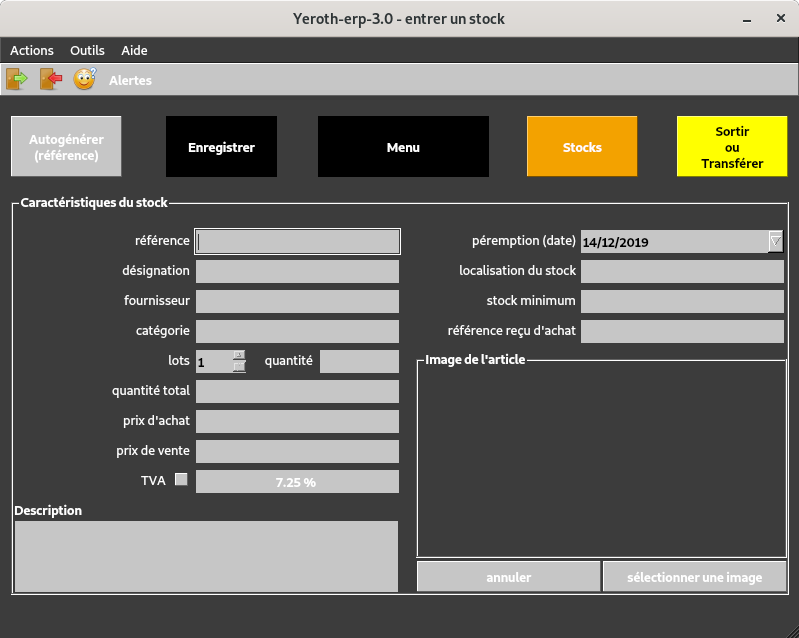
\includegraphics[scale=0.63]{images/yeren-fenetre-entrer.png}
		  \caption{Le formulaire vide pour entrer un stock.}
		  \label{fig:formulaire-entrer-1}
		  \end{figure}
	      
	      \newpage
	      
	\item \textcolor{purplish}{$\mathbf{2^{\text{\`eme}}}$ \textbf{m\'ethode}}
		\begin{enumerate}[1)]
			\item \`A partir de la fen\^etre d'acceuil
			(voir figure~\ref{fig:yeren-fenetre-patron}),
			cliquez sur le boutton \bouton{Stocks}
			\item ensuite, s\'electionnez un stock en cliquant dessus une fois
			\item enfin, cliquez sur le le boutton \bouton{Entrer un stock}.\\
		\end{enumerate}				
		
		L\`a vous obtenez un formulaire partiellement rempli
	    avec les donn\'ees r\'eutilisables du stock s\'electionn\'e.
	    Le formulaire que vous obtenez est celui de la
	    figure~\ref{fig:formulaire-entrer-2}.\\
	    
	    \begin{figure}[!htbp]
		\centering
		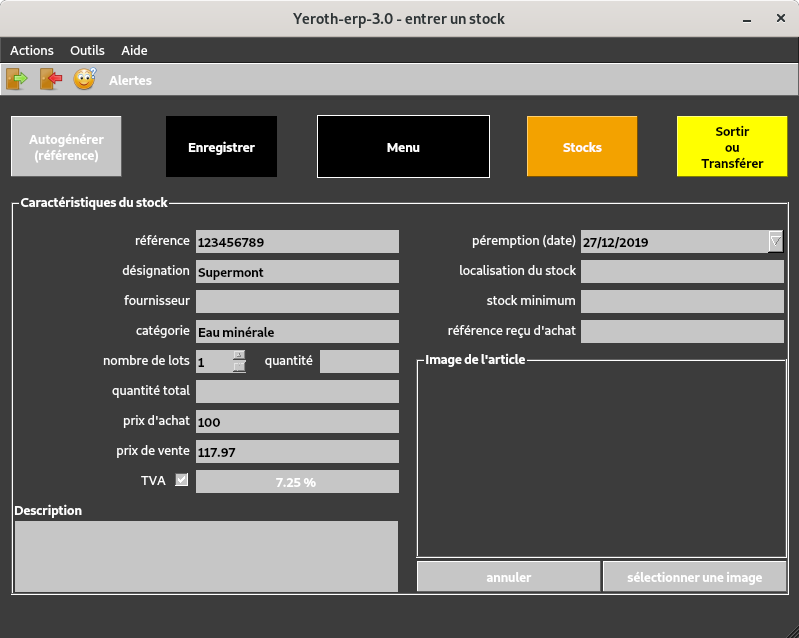
\includegraphics[scale=0.63]{images/yeren-fenetre-entrer-2.png}
		\caption{Le formulaire partiellement rempli pour entrer un nouveau stock.}
		\label{fig:formulaire-entrer-2}
		\end{figure}
\end{itemize}

\newpage

%-----------------------------------------------------------

\nxsection{Lister les stocks}
\index{fiche des stocks}
\index{lister les stocks}
\index{strat\'egie de gestions des stocks}
\index{visualiser la fiche des stocks}
\index{visualiser la liste des stocks}

La figure~\ref{fig:fenetre-lister} illustre la fen\^etre
d'acceuil de \yeren pour lister les stocks.

Le titre de cette fen\^etre explicite la strat\'egie
de gestion des stocks utilis\'ee pour vendre ou
sortir des articles: \dpfdpo.\\

\begin{figure}[!htbp]
\centering
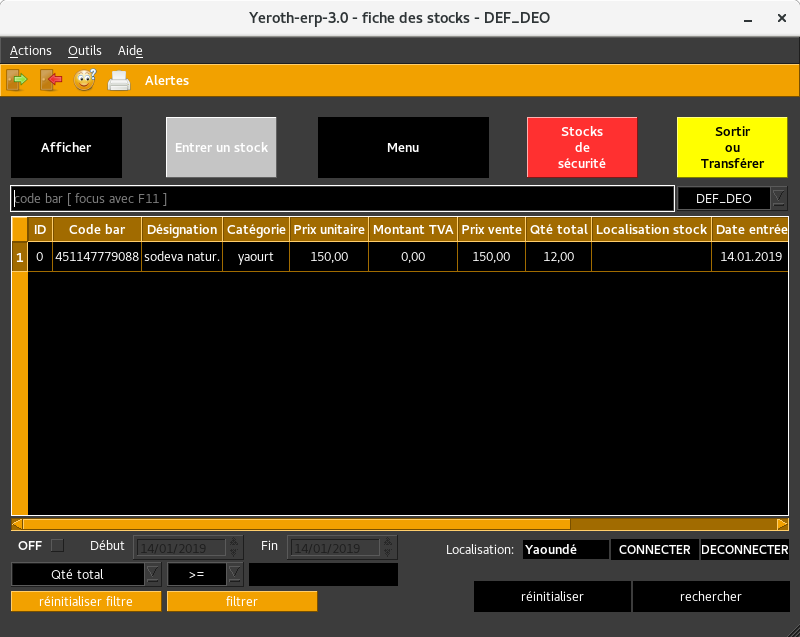
\includegraphics[scale=0.63]{images/yeren-fenetre-lister.png}
\caption{La fen\^etre pour lister les stocks.}
\label{fig:fenetre-lister}
\end{figure}

\subsection{Les stocks list\'es en rouge}
Les stocks list\'es en \textcolor{firebrickred}{rouge} dans
la colone ''Quantit\'e en stock'' sont ceux dont la quantit\'e
minimale en stock a \'et\'e atteinte.

Les stocks list\'es en \textcolor{firebrickred}{rouge} dans
la colone ''Date de p\'eremption'' sont ceux dont la date de
p\'eremption a \'et\'e atteinte.

\subsection{Les stocks list\'es en vert}
Les stocks list\'es en \textcolor{medgreen}{vert} dans la
colone ''Date de p\'eremption'' sont ceux qui ont \'et\'e
s\'electionn\'es pour la vente par l'algorithme correspondant:
\dpfdpo dans le cas de la figure~\ref{fig:fenetre-lister}.

\subsection{Lister les stocks avec le r\^ole \magasinier}
Pour le \role \magasinier, il existe deux m\'ethodes pour
lister les stocks dans \yeren \`a partir de la fen\^etre
d'acceuil (figure~\ref{fig:yeren-fenetre-magasinier}): 

\begin{itemize}[\mycheckmark{purplish}]
	\item \textcolor{purplish}{$\mathbf{1^{\text{\`ere}}}$ \textbf{m\'ethode}}\\
		cliquez sur le bouton \bouton{Stocks} dans le menu
		d\'eroulant \textbf{Actions}\\

	\item \textcolor{purplish}{$\mathbf{2^{\text{\`eme}}}$ \textbf{m\'ethode}}\\
		cliquez sur le bouton \bouton{Stocks} de la de la fen\^etre d'acceuil.
\end{itemize}

\subsection{Lister les stocks avec le r\^ole \manager}
Pour le \role \manager, il existe deux m\'ethodes pour
lister les stocks dans \yeren \`a partir de la fen\^etre
d'acceuil (figure~\ref{fig:yeren-fenetre-patron}): 

\begin{itemize}[\mycheckmark{purplish}]
	\item \textcolor{purplish}{$\mathbf{1^{\text{\`ere}}}$ \textbf{m\'ethode}}\\
		cliquez sur le bouton \bouton{Stocks} dans le menu
		d\'eroulant \textbf{Actions}\\

	\item \textcolor{purplish}{$\mathbf{2^{\text{\`eme}}}$ \textbf{m\'ethode}}\\
		cliquez sur le bouton \bouton{Stocks} de la de la fen\^etre d'acceuil.
\end{itemize}

\subsection{Lister les stocks avec le r\^ole \caissier}
Pour le \role \caissier, il suffit de cliquer sur le lien
'\textbf{Lister les Stocks}' dans la barre de menu
de la fen\^etre de la vente (figure~\ref{fig:fenetre-vendre}).

%-----------------------------------------------------------
\newpage
\nxsection{Imprimer la fiche des stocks
	au format PDF}\label{sec:imprimer-liste-stocks}
\index{imprimer la fiche des stocks}
\index{imprimer la liste des stocks}

Il existe deux m\'ethodes pour imprimer la liste des
stocks qui appara\^it dans la fen\^etre titr\'ee
'\textbf{Yeren - Lister les stocks}'.

\begin{itemize}[\mycheckmark{purplish}]
	\item \textcolor{purplish}{$\mathbf{1^{\text{\`ere}}}$ \textbf{m\'ethode}}\\
		Cliquez sur le lien '\textbf{Imprimer la fiche des stocks}'
		qui se trouve dans le menu d\'eroulant '\textbf{Outils}'\\

	\item \textcolor{purplish}{$\mathbf{2^{\text{\`eme}}}$ \textbf{m\'ethode}}\\
		Pressez simultan\'ement les boutons \bouton{CTRL}
		et \bouton{P} de votre clavier.\\
\end{itemize}

Un fichier au format PDF ayant la liste des stocks affich\'ee
est alors g\'en\'er\'e.

%-----------------------------------------------------------
%\newpage
\nxsection{Rechercher un article ou un stock}
\index{rechercher un article}
\index{rechercher un stock}

Il existe deux m\'etodes pour rechercher un article / stock:
\begin{itemize}[\mycheckmark{purplish}]
	\item \textcolor{purplish}{$\mathbf{1^{\text{\`ere}}}$ \textbf{m\'ethode}}

	\begin{enumerate}[1)]
		\item cliquez sur le bouton \bouton{rechercher}
		\item ou bien cliquez sur le lien '\textbf{Rechercher un article}'
			dans le menu d\'eroulant \textbf{Outils}.\\
	\end{enumerate}
	
	L'utilisateur est alors conduit vers une petite fen\^etre de
	dialogue ou il peut introduire les mots cl\'es de sa recherche,
	ainsi que les param\`etres optionels suivants: la
	\yerenfield{cat\'egorie du stock}, la \yerenfield{d\'esignation du stock}
	et le \yerenfield{fournisseur du stock}.
	Ceci est illustr\'e dans la figure~\ref{fig:fenetre-rechercher-stock}.\\
	
	\begin{figure}[!htbp]
		\centering
		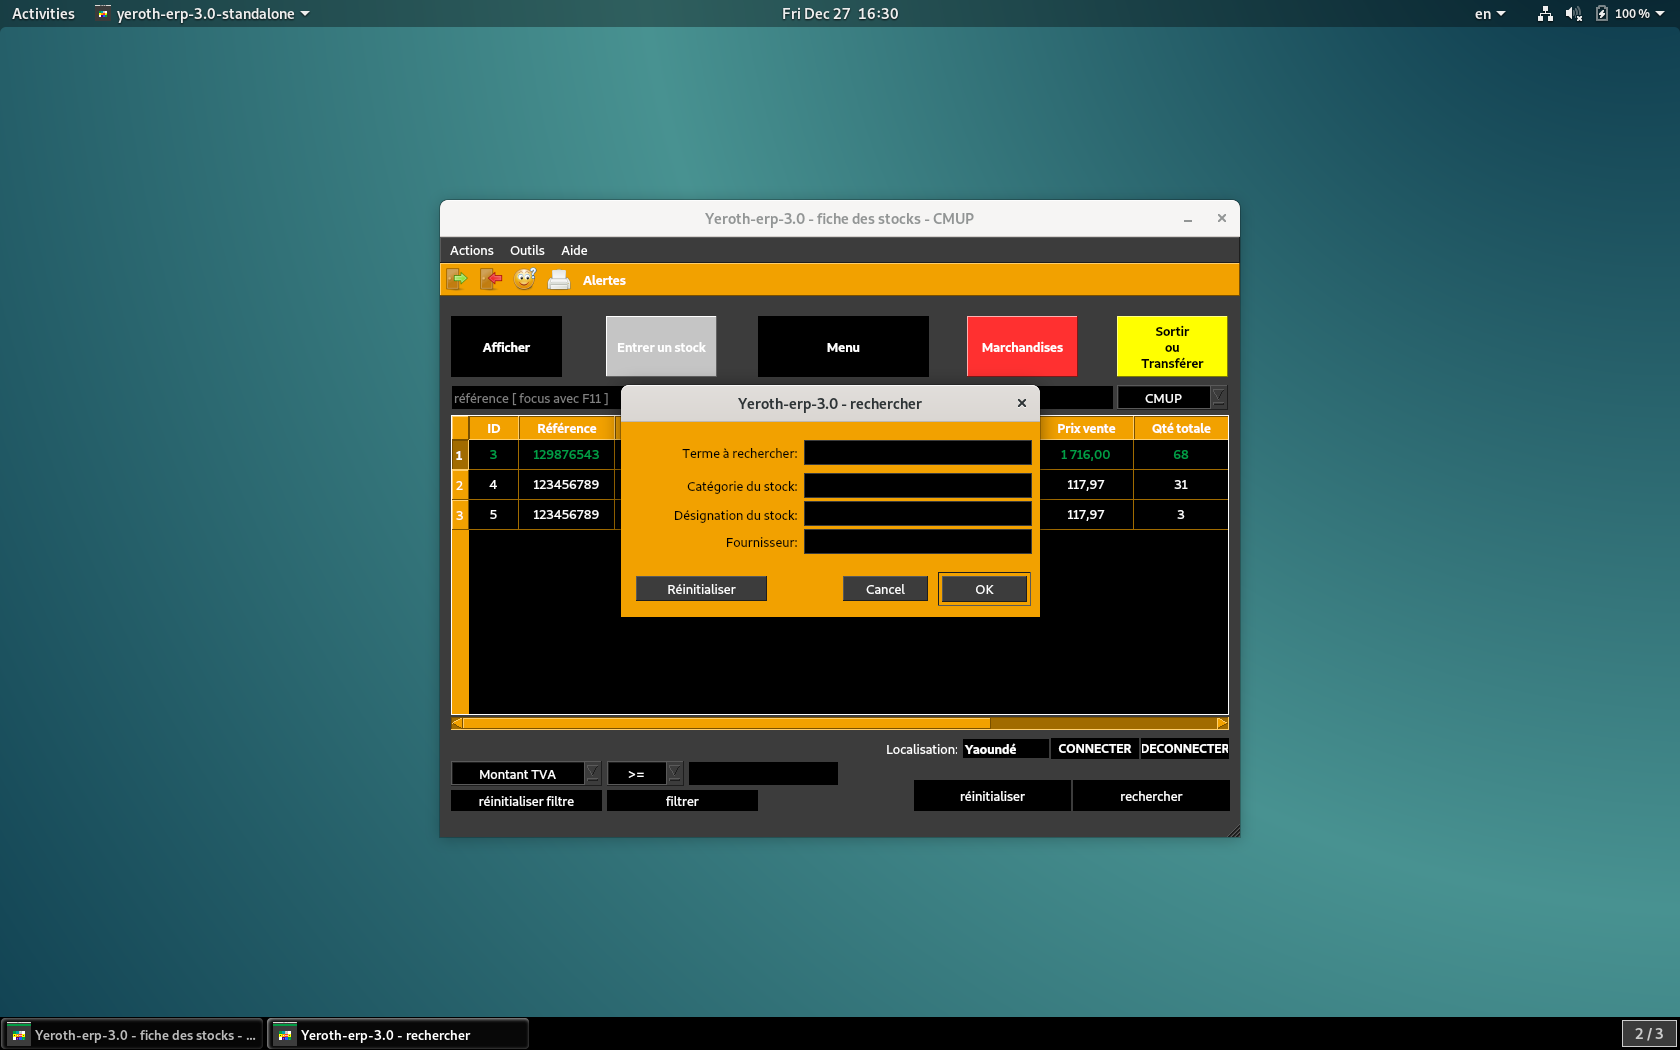
\includegraphics[scale=0.26]{images/yeren-rechercher-un-article.png}
		\caption{La fen\^etre pour rechercher un stock (ou un article).}
		\label{fig:fenetre-rechercher-stock}
	\end{figure}
	
	Pour une recheche efficace, les mots cl\'es doivent \^etre des
	mots ou parcelle de mots qui appara\^issent dans les endroits
	suivant:
	\begin{enumerate}[1)]
		\item la cat\'egorie du stock
		\item la d\'esignation du fournisseur		
		\item la d\'esignation du stock
		\item les mots qui ont \'et\'e introduits dans
			le champs de texte '\textbf{Description}'
			qui appara\^it lorsque l'on entre un nouveau stock
			(voir par example le figure~\ref{fig:formulaire-entrer-2}).
	\end{enumerate}
		
	\newpage	
	
	\item \textcolor{purplish}{$\mathbf{2^{\text{\`eme}}}$ \textbf{m\'ethode}}\\
	L'utilisateur peut aussi entrer la r\'ef\'erence
	du stock recherch\'e dans le champs	de recherche
	situ\'e juste en dessous des boutons
	suivants: \bouton{Afficher}, \bouton{Entrer un nouveau stock},
	\bouton{Menu}, \bouton{Modifier}, et \bouton{Sortir}.\\
		
	\begin{figure}[!htbp]
		\centering
		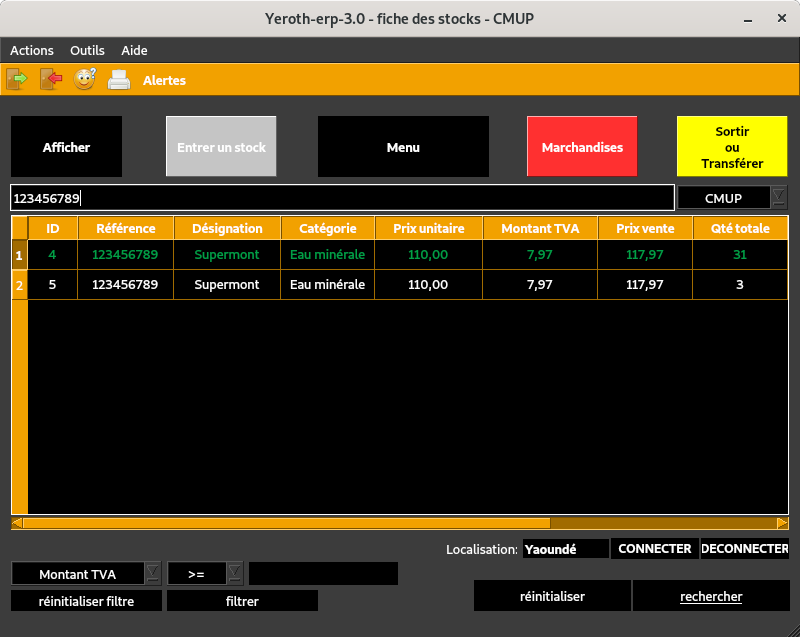
\includegraphics[scale=0.63]{images/yeren-fenetre-rechercher-stock-par-reference.png}
		\caption{Le champs de texte pour
			rechercher les stocks (ou articles) en utilisant
			seulement leur r\'ef\'erence.}\label{fig:yeren-fenetre-rechercher-stock-par-reference}
	\end{figure}
	
	Ceci est illustr\'e dans la figure~\ref{fig:yeren-fenetre-rechercher-stock-par-reference}
	o\`u les stocks ayant la r\'ef\'erence '\textbf{451147779088}'
	ont \'et\'e recherch\'es.\\	
\end{itemize}

Lorsqu'une recherche de stocks (ou d'articles) est active,
le mot 'rechercher' du bouton \bouton{rechercher} et
le lien '\textbf{Rechercher un article}' dans le
menu d\'eroulant '\textbf{Outils}' sont soulign\'es.
	
Le bouton \bouton{r\'einitialiser} ou le lien
'\textbf{R\'einitialiser la recherche}' dans le menu 
d\'eroulant '\textbf{Outils}' permettent d'arr\^eter
la recherche et ainsi d'afficher tous les stocks
\`a nouveau.

%-----------------------------------------------------------
\newpage
\nxsection{Afficher les d\'etails d'un stock}
\index{afficher les d\'etails d'un stock}

La figure~\ref{fig:fenetre-details-stock} illustre
les d\'etails du stock '\textbf{Cola}'.\\

\begin{figure}[!htbp]
	\centering
	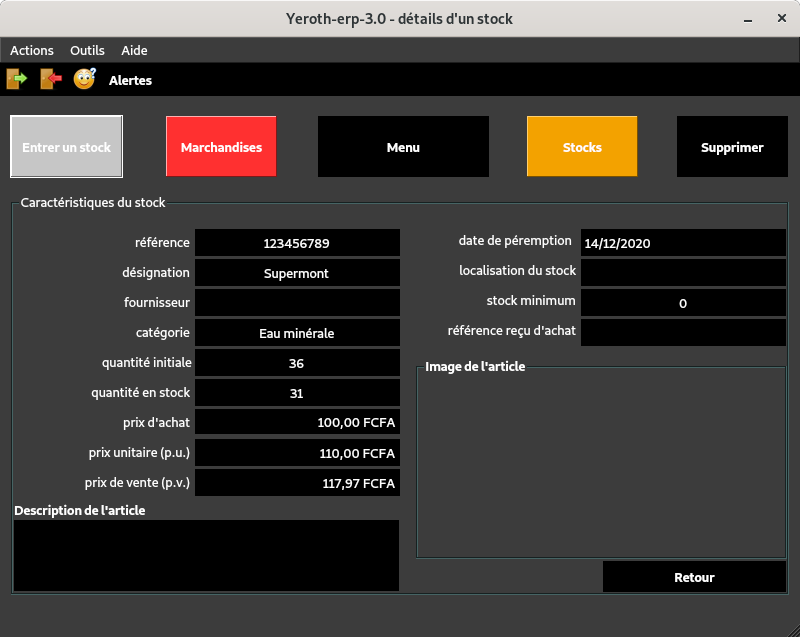
\includegraphics[scale=0.63]{images/yeren-fenetre-detail-stock.png}
	\caption{Une fen\^etre qui pr\'esente les d\'etails d'un stock.}
	\label{fig:fenetre-details-stock}
\end{figure}

Il existe trois m\'ethodes pour afficher les d\'etails
d'un stock:

\begin{itemize}[\mycheckmark{purplish}]
	\item \textcolor{purplish}{$\mathbf{1^{\text{\`ere}}}$ \textbf{m\'ethode}}
		\begin{enumerate}[1)]
			\item s\'electionnez le stock dont vous souhaitez
			afficher les d\'etails en cliquant une fois sur lui
			\` a partir de la fen\^etre '\textbf{lister les stocks}'
			
			\item cliquez ensuite sur le bouton \bouton{Afficher}.	\\
		\end{enumerate}
	
	\item \textcolor{purplish}{$\mathbf{2^{\text{\`eme}}}$ \textbf{m\'ethode}}
		\begin{enumerate}[1)]
			\item s\'electionner le stock dont vous souhaitez
			afficher les d\'etails en cliquant une fois sur lui
			\` a partir de la fen\^etre '\textbf{lister les stocks}'
			
			\item cliquer ensuite sur le lien '\textbf{Afficher ce stock au d\'etail}'
			du menu d\'eroulant \textbf{Actions}.\\
		\end{enumerate}
	
	\item \textcolor{purplish}{$\mathbf{3^{\text{\`eme}}}$ \textbf{m\'ethode}}
		\begin{enumerate}[1)]
			\item s\'electionner le stock dont vous souhaitez
			afficher les d\'etails en cliquant une fois sur lui
			\` a partir de la fen\^etre '\textbf{lister les stocks}'
			
			\item maintener l'indexeur de la souris sur le stock
				s\'electionner et ensuite cliquer sur le bouton
				droit de la souris
			
			\item un menu d\'eroulant s'affiche, cliquer sur
				le lien '\textbf{Afficher ce stock au d\'etail}' du
				menu d\'eroulant qui s'est affich\'e. 
		\end{enumerate}
\end{itemize}

%-----------------------------------------------------------
\newpage
\nxsection{Afficher l'historique d'un stock}
\index{afficher l'historique d'un stock}



%-----------------------------------------------------------
%\newpage
\nxsection{Modifier les d\'etails d'un stock}
\index{modifier les d\'etails d'un stock}

La figure~\ref{fig:yeren-fenetre-modifier-stock}
illustre la fen\^etre pour modifier les d\'etails
du stock '\textbf{Cola}'.\\

\begin{figure}[!htbp]
	\centering
	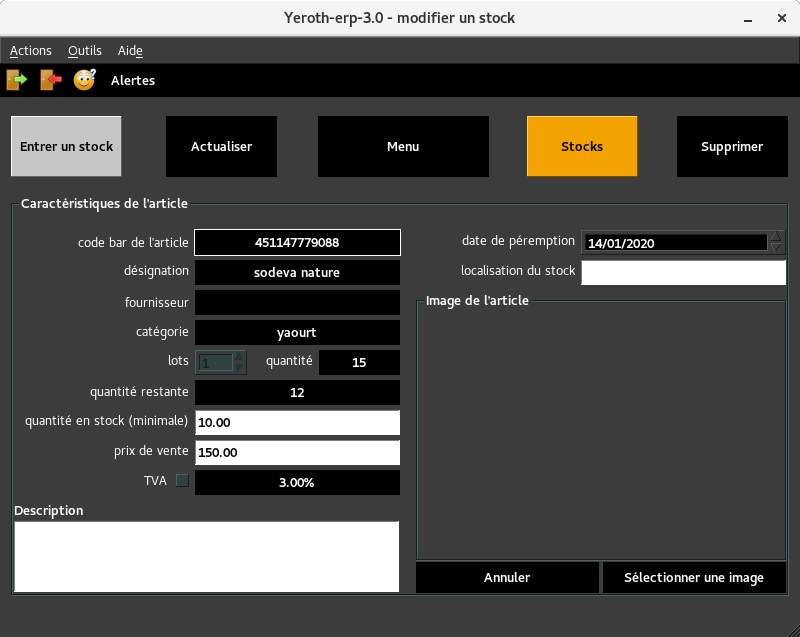
\includegraphics[scale=0.63]{images/yeren-fenetre-modifier-stock.png}
	\caption{Une fen\^etre qui permet la modification des d\'etails d'un stock.}
	\label{fig:yeren-fenetre-modifier-stock}
\end{figure}

Seul les informations suivantes d'un stock peuvent
\^etre modifi\'ees:
\begin{enumerate}[1)]
	\item la date de p\'eremption des articles du stock
	\item la quantit\'e minimale en stock
	\item le prix de vente d'un article du stock.\\
\end{enumerate}

Il existe trois m\'ethodes pour modifier les d\'etails
d'un stock:

\begin{itemize}[\mycheckmark{purplish}]
	\item \textcolor{purplish}{$\mathbf{1^{\text{\`ere}}}$ \textbf{m\'ethode}}
	\begin{enumerate}[1)]
		\item s\'electionner le stock dont vous souhaitez
		modifier les d\'etails en cliquant une fois sur lui
		\` a partir de la fen\^etre '\textbf{lister les stocks}'
		
		\item cliquer ensuite sur le bouton \bouton{Modifier}.	\\
	\end{enumerate}
	
	\item \textcolor{purplish}{$\mathbf{2^{\text{\`eme}}}$ \textbf{m\'ethode}}
	\begin{enumerate}[1)]
		\item s\'electionner le stock dont vous souhaitez
		modifier les d\'etails en cliquant une fois sur lui
		\` a partir de la fen\^etre '\textbf{lister les stocks}'
		
		\item cliquer ensuite sur le lien '\textbf{Modifier ce stock}'
		du menu d\'eroulant \textbf{Actions}.\\
	\end{enumerate}
	
	\item \textcolor{purplish}{$\mathbf{3^{\text{\`eme}}}$ \textbf{m\'ethode}}
	\begin{enumerate}[1)]
		\item s\'electionner le stock dont vous souhaitez
		modifier les d\'etails en cliquant une fois sur lui
		\` a partir de la fen\^etre '\textbf{lister les stocks}'
		
		\item maintener l'indexeur de la souris sur le stock
		s\'electionn\'e et ensuite cliquer sur le bouton
		droit de la souris
		
		\item un menu d\'eroulant s'affiche, cliquer sur
		le lien '\textbf{Modifier ce stock}' du	menu
		d\'eroulant qui s'est affich\'e.\\
	\end{enumerate}
\end{itemize}

%-----------------------------------------------------------

\newpage
\nxsection{Visualiser les articles / stocks p\'erim\'es}
\index{visualiser les articles p\'erim\'es}
\index{visualiser les stocks p\'erim\'es}

La figure~\ref{fig:fenetre-lister-stock-perime} illustre
que la date de p\'eremption du stock 'Cola' ($22$ F\'evrier
$2017$) est d\'epass\'ee.\\

\begin{figure}[!htbp]
	\centering
	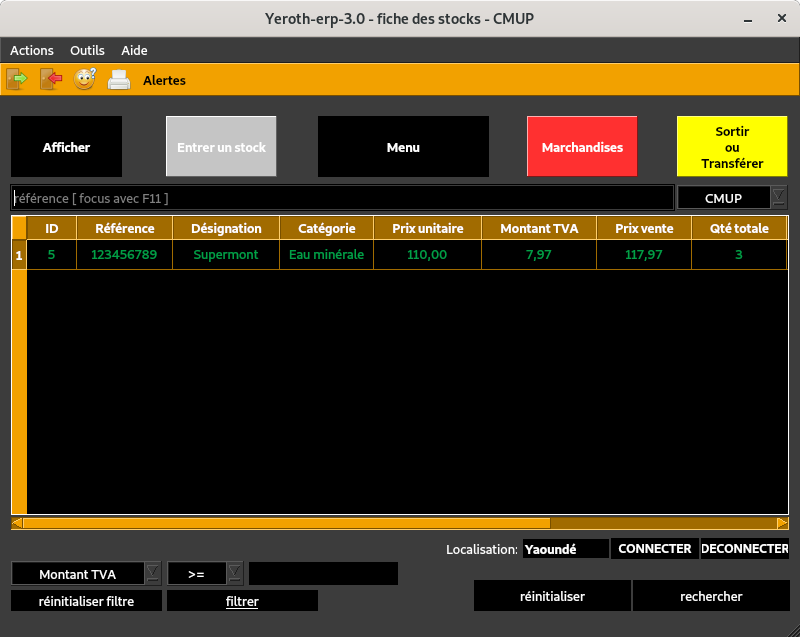
\includegraphics[scale=0.63]{images/yeren-fenetre-stocks-perimes.png}
	\caption{Le stock 'Cola' est p\'erim\'e.}
	\label{fig:fenetre-lister-stock-perime}
\end{figure}

On visualise les stocks p\'erim\'es en allant \`a la fen\^etre
'\textbf{lister les stocks}'. 

Tous les stocks dont la colone '\textbf{Date de
	p\'eremption}' est affich\'ee en 
\textbf{\textcolor{firebrickred}{rouge}} sont p\'erim\'es.

%-----------------------------------------------------------

\newpage
\nxsection{Visualiser les stocks dont la quantit\'e minimale 
	en stock est atteinte}
\index{la quantit\'e minimale en stock est atteinte}

L'utilisateur de \yeren peut d\'efinir une quantit\'e minimale
pour un stock: c'est \emph{le nombre d'articles du stock en dessous
duquel l'entreprise ne devrait pas se retrouver}.

La figure~\ref{fig:fenetre-lister-quantite-minimale} illustre
que la quantit\'e minimale de $50$ articles du stock 'Cola'
est atteinte.\\

\begin{figure}[!htbp]
	\centering
	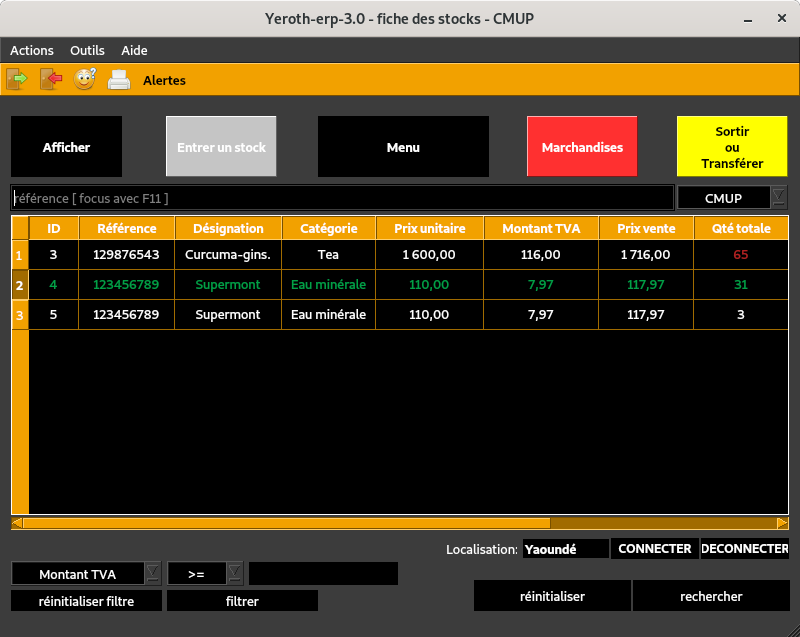
\includegraphics[scale=0.63]{images/yeren-fenetre-stock-minimal-atteint.png}
	\caption{La quantit\'e minimale du stock 'Cola' est atteinte.}
	\label{fig:fenetre-lister-quantite-minimale}
\end{figure}

On visualise les stocks dont la quantit\'e minimale en stock
est atteinte en allant \`a la fen\^etre '\textbf{lister les stocks}'.

Tous les stocks dont la colone '\textbf{Quantit\'e en stock}'
est affich\'ee en \textbf{\textcolor{firebrickred}{rouge}}
ont leur quantit\'e minimale en stock d\'ej\`a ateinte.

%-----------------------------------------------------------

%\newpage
\nxsection{Supprimer un stock}
\index{supprimer un stock}

Il existe deux m\'etodes pour supprimer un stock:
\begin{itemize}[\mycheckmark{purplish}]
	\item \textcolor{purplish}{$\mathbf{1^{\text{\`ere}}}$ \textbf{m\'ethode}}
	
	\begin{enumerate}[1)]
		\item s\'electionner le stock \`a supprimer partir de
		la fen\^etre '\textbf{lister les stocks}'
		
		\item cliquer ensuite sur le lien '\textbf{Supprimer ce stock}'
		dans le menu d\'eroulant \textbf{Actions}.\\
	\end{enumerate}
	
	\item \textcolor{purplish}{$\mathbf{2^{\text{\`eme}}}$ \textbf{m\'ethode}}
	\begin{enumerate}[1)]
		\item s\'electionner le stock \`a supprimer partir de
			la fen\^etre '\textbf{lister les stocks}'
		
		\item maintener l'indexeur de la souris sur le stock
			s\'electionn\'e et ensuite cliquer sur le bouton
			droit de la souris
				
		\item un menu d\'eroulant s'affiche, cliquer sur
			le lien '\textbf{Supprimer ce stock}' du menu
			d\'eroulant qui s'est affich\'e. \\
	\end{enumerate}	
\end{itemize}

Le stock supprim\'e n'est plus affich\'e.
